\documentclass[11pt]{article}

\usepackage[margin=1in]{geometry}
\usepackage{amsmath,amssymb,amsthm}
\usepackage{booktabs}
\usepackage{graphicx}
\usepackage{caption}
\usepackage[colorlinks=true,linkcolor=blue,citecolor=blue,urlcolor=blue]{hyperref}
\usepackage{enumitem}

\newtheorem{proposition}{Proposition}
\newtheorem{definition}{Definition}
\newtheorem{corollary}{Corollary}

\title{Is Sector Rotation Predictable?\\
A Markov-Chain Test Against the Correct Random-Matrix Null}

\author{Chan Tsz Him Chris}
\date{July 23, 2026}

\begin{document}
\maketitle

\begin{abstract}
We formalize ``sector leadership rotation'' in the S\&P 500 as a discrete-time Markov chain and ask whether the resulting dynamics contain genuine predictive structure or are statistically indistinguishable from noise. We first address a construction problem that is often skipped: a matrix of pairwise conditional probabilities $\mathbb P(B\!\uparrow \mid A\!\downarrow)$ is not a valid transition matrix, because no single categorical state is defined and the row-sum-to-one constraint is violated. We resolve this by defining the state as the sector with the worst same-period return (the \emph{laggard}) and estimate the resulting chain on eleven SPDR sector ETFs using CRSP daily data, 2010--2024. We characterize the chain's ergodic properties (irreducibility, aperiodicity, stationary distribution, recurrence and hitting times) and its spectral structure (eigenvalues, spectral gap, mixing time, complex eigenvalue pairs). The central methodological contribution is testing this spectral structure against the \emph{correct} null model for a row-stochastic matrix --- the circular law for random Markov matrices \cite{bordenave2012} --- rather than the Marchenko--Pastur law, which applies to sample covariance matrices and is structurally inapplicable here. Using both a closed-form disk-radius approximation and a 5{,}000-replication permutation bootstrap, we find that every non-Perron eigenvalue of the estimated chain is statistically indistinguishable from what a random stochastic matrix of the same size would produce. We show this null result is consistent with the microstructure of the underlying products: cap-weighted sector ETFs, unlike equal-weight or daily-rebalanced leveraged funds, embed no mechanical rebalancing flow that would force mean-reverting or momentum-driven serial structure onto the laggard sequence.
\end{abstract}

\clearpage
\section{Introduction}

On a day when a large semiconductor name disappoints, the technology sector sells off and capital appears to rotate into other leaders (financials, say, or utilities). Traders describe this informally as ``sector rotation,'' and the natural instinct is to encode it as a matrix of conditional probabilities: given that sector $A$ fell today, what is the probability sector $B$ leads tomorrow? That instinct does not survive contact with the actual definition of a Markov chain.

On any given day \emph{all} eleven sectors move simultaneously; there is no single ``current state'' the market occupies, so a chain cannot be defined directly on the vector of sector returns without first collapsing it to a categorical label. And even a well-intentioned analyst who forces a $\mathbb P(B\!\uparrow \mid A\!\downarrow)$ table to look like a transition matrix will find its rows do not actually sum to one, because the events ``$B$ rises'' for different $B$ are not mutually exclusive.

This paper works through the correct construction end to end: a cleanly defined single-state-per-period object, a transition law estimated from real CRSP sector-ETF data, a full characterization as a Markov chain (stationarity, recurrence, hitting times, spectral gap, cyclical structure), and a test of whether the resulting spectral structure is real or a finite-sample artifact, using the null model actually appropriate for a row-stochastic matrix instead of the one (Marchenko--Pastur) reflexively reached for in the empirical finance literature. We close by connecting the statistical result to a microstructural mechanism: whether an index's rebalancing rule injects mean-reverting or momentum flow into its constituent dynamics, and why cap-weighted products should not be expected to.

\clearpage
\section{Related Work}
\label{sec:related}

This paper sits at the intersection of three literatures that are not usually brought together: regime-switching models of markets, the empirical evidence on sector rotation as a strategy, and random matrix theory applied to financial data.

\subsection{Regime-switching and Markov models in finance}

Treating a financial time series as governed by a small number of discrete, unobserved states goes back to \cite{hamilton1989}, whose Markov-switching autoregression became the standard tool for dating business-cycle regimes from macroeconomic data. That literature typically models a \emph{latent} state (e.g.\ ``expansion'' vs.\ ``recession'') inferred via maximum likelihood from an observed continuous series. Our setup differs in kind, not just application: the state $S_t$ (the daily laggard sector) is directly \emph{observed}, not inferred, which is what allows the transition matrix to be estimated by simple counting (Section~\ref{sec:estimation}) rather than by filtering. This also means the two constructions face different failure modes: Hamilton-style regime models must contend with state misclassification from the estimation procedure itself, while our chain's main threat to validity is the construction problem addressed in Section~\ref{sec:state}, defining a legitimate single state per period in the first place.

\subsection{Sector rotation as an empirical strategy}

``Sector rotation'' is better documented as a practitioner heuristic than as a robust empirical regularity. \cite{moskowitzgrinblatt1999} showed that industry-level momentum accounts for much of the individual-stock momentum anomaly, i.e.\ that sectors as a group do exhibit return persistence at monthly-to-annual horizons. Tested directly as a market-timing strategy, however, the evidence is considerably weaker: \cite{jacobsenetal2009} find that a sector-rotation strategy with \emph{perfect foresight} of the business-cycle stage, and no transaction costs, would have generated at best a 2.3\% annual outperformance over 1948--2007, an upper bound that erodes quickly once foresight and costs are made realistic. More recently, \cite{molchanovstangl2024} report no systematic evidence of the sector outperformance patterns conventional sector-rotation wisdom predicts across business-cycle stages at all. Our result is a different, and in one sense more basic, negative finding: these prior papers ask whether a business-cycle-\emph{timed} sector rotation strategy is profitable, while we ask whether the day-to-day \emph{identity} of the laggard sector carries any Markov memory whatsoever, independent of any macro-timing signal. Given the monthly-momentum evidence of \cite{moskowitzgrinblatt1999}, the two horizons need not agree, and our null result at the one-day horizon is not in tension with theirs at the monthly one.

\subsection{Random matrix theory in finance}

The idea that a financial correlation or transition matrix should be benchmarked against its random-matrix null, rather than interpreted directly, dates to \cite{lalouxetal1999} and \cite{plerouetal2000}, who independently showed that the great majority of eigenvalues of empirical stock-return correlation matrices are statistically indistinguishable from the Marchenko--Pastur spectrum of a matrix built from pure noise; see \cite{bouchaudpotters2009} for a broader review. That entire line of work, however, benchmarks \emph{symmetric} correlation matrices against Marchenko--Pastur, which is exactly the null we show in Section~\ref{sec:rmt} does \emph{not} apply to a non-symmetric, row-stochastic transition matrix. Our use of the circular law for random Markov matrices \cite{bordenave2012} in its place is the natural analogue of the Laloux--Plerou research program for the object we actually estimate, and, as far as we are aware, sector-rotation dynamics have not previously been tested against it.

\clearpage
\section{Constructing a Legitimate State Space}
\label{sec:state}

\subsection{Why a pairwise conditional-probability matrix fails}

Consider a matrix $M$ with entries $M_{AB} = \mathbb P(B\!\uparrow \mid A\!\downarrow)$, estimated across all sector pairs. It fails as a Markov transition matrix for two separate reasons.

\emph{(i) No single current state.} A Markov chain requires a well-defined state $S_t$ that the system occupies at each time $t$, with transitions $S_t \to S_{t+1}$. Every period, though, all $n$ sectors move at once. The ``state'' of the market on day $t$ is really an $n$-dimensional return vector $(r_{1,t},\dots,r_{n,t})$, not a single categorical label, and $M$ implicitly treats \emph{every sector} as simultaneously ``the'' current state. That is incoherent: $A$ falling does not preclude nine other sectors from also falling or rising in the same period, so there is no unique antecedent to condition on.

\emph{(ii) Rows need not sum to one.} Even fixing a reference sector $A$, the events ``$B$ rises'' for different $B\neq A$ are not mutually exclusive: on a given day multiple sectors can rise together, or none can. Summing $\mathbb P(B\!\uparrow\mid A\!\downarrow)$ over $B$ therefore double-counts joint outcomes and violates the law of total probability; $\sum_B M_{AB}$ can exceed or fall short of 1 depending on the realized correlation structure. Forcing normalization onto such a table produces something row-stochastic by fiat, with no meaning as a transition law.

\subsection{Resolution: a single categorical state}

We collapse each period to exactly one state by defining
\begin{equation}
S_t \;=\; \arg\min_{i \in \{1,\dots,n\}} r_{i,t},
\end{equation}
the \emph{laggard sector} (the sector with the worst return in period $t$). Because $\arg\min$ selects a unique index (ties aside, which do not occur in our continuous return data), the market occupies exactly one of $n$ states each period, and
\begin{equation}
P_{ij} \;=\; \mathbb P(S_{t+1} = j \mid S_t = i)
\end{equation}
is now a genuine transition probability. (An analogous construction with $\arg\max$ defines a ``leader'' chain; we use the laggard definition throughout, following the source problem set this paper extends.)

\begin{definition}[Row-stochastic matrix]
An $n\times n$ matrix $P$ is a (row-)stochastic transition matrix if and only if
\begin{equation}
\text{(1)}\quad P_{ij} \ge 0 \ \ \forall i,j, \qquad\qquad \text{(2)}\quad \sum_{j=1}^n P_{ij} = 1 \ \ \forall i.
\end{equation}
\end{definition}

Unlike $M$ above, $P$ satisfies both conditions by construction: at each $t$ exactly one transition $S_t \to S_{t+1}$ is observed, so the counts $n_{ij}$ used to estimate $P$ (Section~\ref{sec:estimation}) partition the sample exhaustively and $\sum_j P_{ij}=1$ follows automatically. A conditional-probability contingency table like $M$ remains the right tool for a different question --- \emph{co-movement}, e.g. ``how often does $B$ rise alongside $A$ falling'' --- but it answers a static association question, not a dynamic state-transition question, and the two objects should not be conflated.

\clearpage
\section{Data}
\label{sec:data}

We use the eleven SPDR Select Sector ETFs as tradable proxies for the GICS sectors: Technology (XLK), Health Care (XLV), Financials (XLF), Consumer Discretionary (XLY), Communication Services (XLC), Industrials (XLI), Consumer Staples (XLP), Energy (XLE), Utilities (XLU), Real Estate (XLRE), and Materials (XLB). Daily total returns (CRSP \texttt{dsf}, split- and dividend-adjusted) are pulled via WRDS for 2010-01-01 through 2024-12-31, matched to PERMNOs via \texttt{crsp.stocknames}, yielding 37{,}934 sector-day observations.

Sanity checks: 2 missing return observations (0.005\% of the sample), zero returns exceeding 50\% in magnitude, and a 0.995 correlation between CRSP's total return field and a price-only return reconstructed independently from the price series (the residual gap is attributable to dividends, which CRSP's total return correctly includes). All 11 sectors are present with zero duplicate (sector, date) pairs.

The panel is unbalanced: XLC (Communication Services) launched in June 2018 and XLRE (Real Estate) in October 2015, while the remaining nine sectors trade from January 2010. We therefore restrict the Markov-chain analysis to the \emph{common period}, 2018-06-20 through 2024-12-31 (1{,}644 trading days, 1{,}643 transitions), where all 11 states are simultaneously well-defined. A weekly-frequency series (Friday-to-Friday compounded returns, 342 weeks) is used only for the data-adequacy discussion in Section~\ref{sec:sparsity}.

\clearpage
\section{Estimation: Maximum Likelihood and Smoothing}
\label{sec:estimation}

\subsection{A worked example}

A small hand-worked three-state (Technology, Financials, Energy) example illustrating this estimation and smoothing procedure is given in Appendix~\ref{app:toy}.

\subsection{Free parameters and data adequacy}
\label{sec:sparsity}

For a general $n$-state chain, $P$ has $n^2$ entries but each row loses one degree of freedom to the sum-to-one constraint, leaving
\begin{equation}
\#\text{free parameters} = n(n-1).
\end{equation}
For our $n=11$ sector universe this is $110$. A standard rule of thumb calls for roughly 10--20 observed transitions per parameter for reliable MLE estimation, i.e.\ 1{,}100--2{,}200 transitions. Our common-period daily sample provides 1{,}643 transitions (14.9 per parameter); the weekly sample provides only 341 (3.1 per parameter) --- comfortably adequate at daily frequency, badly under-identified at weekly frequency. This motivates two design choices: daily data over weekly, and, were data even scarcer, a small number of macro regimes (e.g.\ $k=3$) instead of $n=11$ raw sectors, since $k(k-1)=6$ free parameters would make even the weekly sample generous (56.8 transitions per parameter).

\subsection{Laplace smoothing}

We apply additive (Laplace) smoothing,
\begin{equation}
\tilde P_{ij} \;=\; \frac{n_{ij}+\alpha}{n_{i\cdot}+\alpha n}, \qquad \alpha = 1,
\end{equation}
to every row. Applied to the toy Energy row ($n_{E\cdot}=2$, $n=3$ states), this gives
\begin{equation}
\tilde P_{E,\cdot} = \left(\frac{1+1}{2+3},\ \frac{1+1}{2+3},\ \frac{0+1}{2+3}\right) = (0.400,\ 0.400,\ 0.200)
\end{equation}
in $(T,F,E)$ order, replacing the zero with a small positive probability. Removing that zero entry has real consequences for the estimator: a zero can render the estimated chain \emph{reducible} in finite samples, because if some state $j$ is never reached from $i$, no power $P^k$ can guarantee positivity from $i$ to $j$, and this would block the Perron--Frobenius guarantees (unique stationary distribution, convergence to it) that the remainder of the paper relies on. We apply the same $\alpha=1$ smoothing to the empirical 11-sector count matrix before any spectral analysis; the full smoothed matrix appears in Table~\ref{tab:daily_ptilde} (Appendix~\ref{app:matrices}), with raw counts in Table~\ref{tab:daily_counts}.

\clearpage
\section{Ergodic Properties}
\label{sec:ergodic}

\begin{proposition}[Perron--Frobenius, see e.g.\ \cite{seneta2006,norris1998}]
If $P$ is irreducible (some power $P^k$ is entrywise positive) and aperiodic (the greatest common divisor of return-time lengths at every state is 1), then $P$ has a unique stationary distribution $\pi$ satisfying $\pi P = \pi$, $\sum_i \pi_i = 1$, $\pi_i>0\ \forall i$, and $P^t \to \mathbf 1 \pi$ as $t\to\infty$ from every initial distribution.
\end{proposition}

We verify both conditions directly on the empirical daily smoothed matrix $\tilde P$: every diagonal entry $\tilde P_{ii}>0$ (Table~\ref{tab:daily_ptilde}), which makes the chain aperiodic by inspection, and $\tilde P$ itself is entrywise positive, irreducible already at $k=1$ with minimum entry $0.0179$. Both hold, so the chain is ergodic and $\pi$ is unique.

\subsection{Toy example}

The stationary-distribution and recurrence-time calculations below are illustrated first on a small hand-worked three-state example in Appendix~\ref{app:toy}.

\subsection{Empirical stationary distribution and recurrence times}

For the 11-sector daily chain, $\pi$ is obtained as the (normalized) left eigenvector of $\tilde P$ associated with eigenvalue 1; we verify $\|\pi \tilde P - \pi\| = 1.5\times10^{-16}$, i.e.\ numerically exact. Table~\ref{tab:pi} reports $\pi$ and the mean recurrence time $\mu_i = 1/\pi_i$ (Kac's lemma \cite{kemenysnell1976}) for every sector. Energy is by far the most frequent laggard ($\pi=0.226$, recurring every 4.4 trading days on average); Industrials is the rarest ($\pi=0.032$, recurring only every 31.5 days).

\begin{table}[htbp]\centering
\caption{Stationary distribution $\pi$ and mean recurrence time $\mu_i=1/\pi_i$, daily smoothed chain, common period.}
\label{tab:pi}
\begin{tabular}{lcc}
\toprule
Sector & $\pi_i$ & $\mu_i$ (days) \\
\midrule
Energy & 0.2256 & 4.4 \\
Utilities & 0.1327 & 7.5 \\
Technology & 0.1015 & 9.9 \\
Real Estate & 0.1009 & 9.9 \\
Communication & 0.0822 & 12.2 \\
Consumer Disc. & 0.0743 & 13.5 \\
Health Care & 0.0680 & 14.7 \\
Consumer Staples & 0.0669 & 15.0 \\
Materials & 0.0612 & 16.3 \\
Financials & 0.0550 & 18.2 \\
Industrials & 0.0317 & 31.5 \\
\bottomrule
\end{tabular}
\end{table}

\subsection{Hitting times}

The expected first-passage (hitting) time $h_{ij} = \mathbb E[\min\{t\ge0 : S_t=j\} \mid S_0=i]$ solves the linear system
\begin{equation}
h_{ij} = 1 + \sum_{k} \tilde P_{ik}\, h_{kj} \quad (i \ne j), \qquad h_{jj}=0,
\end{equation}
solved separately for each target $j$ as an $(n-1)$-dimensional linear system with a boundary row fixing $h_{jj}=0$. The full $11\times11$ hitting-time matrix is reported in Table~\ref{tab:hitting} (Appendix~\ref{app:matrices}); consistent with $\pi$, Energy is reached fastest from any starting sector (mean hitting time 4.1 days) and Industrials slowest (28.3 days).

\clearpage
\section{Spectral Analysis}
\label{sec:spectral}

\subsection{Toy example: spectral gap and a complex eigenvalue pair}

The spectral-gap and complex-eigenvalue calculations below are illustrated first on a small hand-worked three-state example, including a cyclic case with a complex eigenvalue pair, in Appendix~\ref{app:toy}.

\subsection{Empirical spectrum}

The eigenvalues of the empirical daily $\tilde P$, sorted by modulus, are given in Table~\ref{tab:eig}. The Perron eigenvalue is $\lambda_0=1$ exactly (verified to machine precision), consistent with Perron--Frobenius. The second-largest modulus is $|\lambda_1|=0.0844$, giving spectral gap
\begin{equation}
\gamma = 1 - |\lambda_1| = 0.9156,
\end{equation}
relaxation time $1/\gamma \approx 1.09$ trading days, and a total-variation mixing time $\tau_{\text{mix}}(\varepsilon{=}0.01)\approx 8.8$ days using the standard bound $\|P^t(x,\cdot)-\pi\|_{TV} \le |\lambda_1|^t/(2\sqrt{\pi_{\min}})$ \cite{levinperes2017}. Starting from Technology, the total-variation distance to $\pi$ falls from $0.076$ at $t=1$ to $2\times10^{-6}$ by $t=5$: the chain mixes almost immediately. Three complex conjugate eigenvalue pairs are present (Table~\ref{tab:eig}), with implied cycle periods between 2.3 and 14.2 trading days, but all are damped to under 1\% of their initial amplitude within two steps. Section~\ref{sec:rmt} tests formally whether any of this is cyclical structure or noise.

\begin{table}[htbp]\centering
\caption{Eigenvalues of the daily smoothed transition matrix $\tilde P$ (11 sectors, common period), sorted by modulus.}
\label{tab:eig}
\begin{tabular}{lccl}
\toprule
$\lambda$ & Value & $|\lambda|$ & Note \\
\midrule
$\lambda_0$ & $1.0000$ & $1.0000$ & Perron root \\
$\lambda_1$ & $0.0844$ & $0.0844$ & real \\
$\lambda_{2,3}$ & $-0.0116 \pm 0.0678i$ & $0.0688$ & complex pair, period $\approx3.6$ days \\
$\lambda_{4,5}$ & $-0.0482 \pm 0.0208i$ & $0.0525$ & complex pair, period $\approx2.3$ days \\
$\lambda_6$ & $-0.0380$ & $0.0380$ & real \\
$\lambda_{7,8}$ & $0.0250 \pm 0.0118i$ & $0.0276$ & complex pair, period $\approx14.2$ days \\
$\lambda_9$ & $0.0105$ & $0.0105$ & real \\
$\lambda_{10}$ & $0.0015$ & $0.0015$ & real \\
\bottomrule
\end{tabular}
\end{table}

\clearpage
\section{The Correct Random-Matrix Null}
\label{sec:rmt}

The eigenvalues in Table~\ref{tab:eig} are small in absolute terms, but ``small'' is not itself a statistical statement: it says nothing without a null distribution to compare against.

\subsection{Why Marchenko--Pastur does not apply}

The Marchenko--Pastur (MP) law \cite{marchenkopastur1967} describes the limiting eigenvalue distribution of a sample covariance matrix $\frac1T XX^\top$, where $X$ is a $p\times T$ matrix of i.i.d.\ mean-zero entries, in the joint limit $p,T\to\infty$ with $p/T\to c\in(0,\infty)$. Four structural mismatches make it inapplicable to our transition matrix $\tilde P$:
\begin{enumerate}[label=(\roman*)]
\item $\frac1T XX^\top$ is symmetric and positive semi-definite; $\tilde P$ is neither --- it is a general (non-symmetric) row-stochastic matrix.
\item MP entries are (asymptotically) i.i.d.\ across the whole matrix; the entries within a row of $\tilde P$ are \emph{not} independent, since they are constrained to sum to 1.
\item $\tilde P$ has a structural eigenvalue pinned exactly at $\lambda_0=1$ by the row-stochasticity constraint; the MP spectrum has no such fixed point and is centered differently depending on the aspect ratio $c$.
\item MP is an asymptotic result requiring $p,T\to\infty$ jointly; our matrix is $n=11$, nowhere near that regime, and $p/T$ has no natural analogue here (there is no ``covariance sample size'' underlying $\tilde P$'s row constraint).
\end{enumerate}

\subsection{Circular law for random Markov matrices}

The appropriate null instead comes from \cite{bordenave2012}: for an $n\times n$ matrix with i.i.d.\ rows drawn uniformly on the probability simplex (equivalently, $\mathrm{Dirichlet}(1,\dots,1)$), the Perron eigenvalue is exactly 1 by construction, and as $n\to\infty$ the remaining $n-1$ eigenvalues become asymptotically uniformly distributed over a disk in the complex plane centered at the origin with radius
\begin{equation}
r_n \;\approx\; \frac{1}{\sqrt n}.
\end{equation}
For $n=11$, $r_{11} = 1/\sqrt{11} \approx 0.3015$. We cross-check this asymptotic formula against a direct Monte Carlo simulation: 1{,}000 independently drawn $11\times11$ Dirichlet-row stochastic matrices yield 10{,}000 non-Perron eigenvalues with mean modulus $0.179$, 95th-percentile modulus $0.308$, and 99th-percentile modulus $0.367$ (Figure~\ref{fig:circular}), close to the asymptotic radius even at this modest $n$, with the expected upward finite-sample correction at the tail.

\subsection{Toy example: a genuine signal}

Applying this null to the toy cyclic example of Appendix~\ref{app:toy}: $|\lambda_2|\approx0.70$ is far outside the disk of radius $\approx0.30$, so that hypothetical chain \emph{would} constitute a statistically genuine cyclical signal.

\subsection{Empirical result: no detectable signal}

Every non-Perron eigenvalue of the empirical $\tilde P$ has modulus $\le0.084$ (Table~\ref{tab:eig}), well inside the $\approx0.30$ noise disk. Figure~\ref{fig:circular} overlays the observed spectrum on the simulated circular-law cloud; all eigenvalues sit deep in the bulk.

\begin{figure}[htbp]\centering
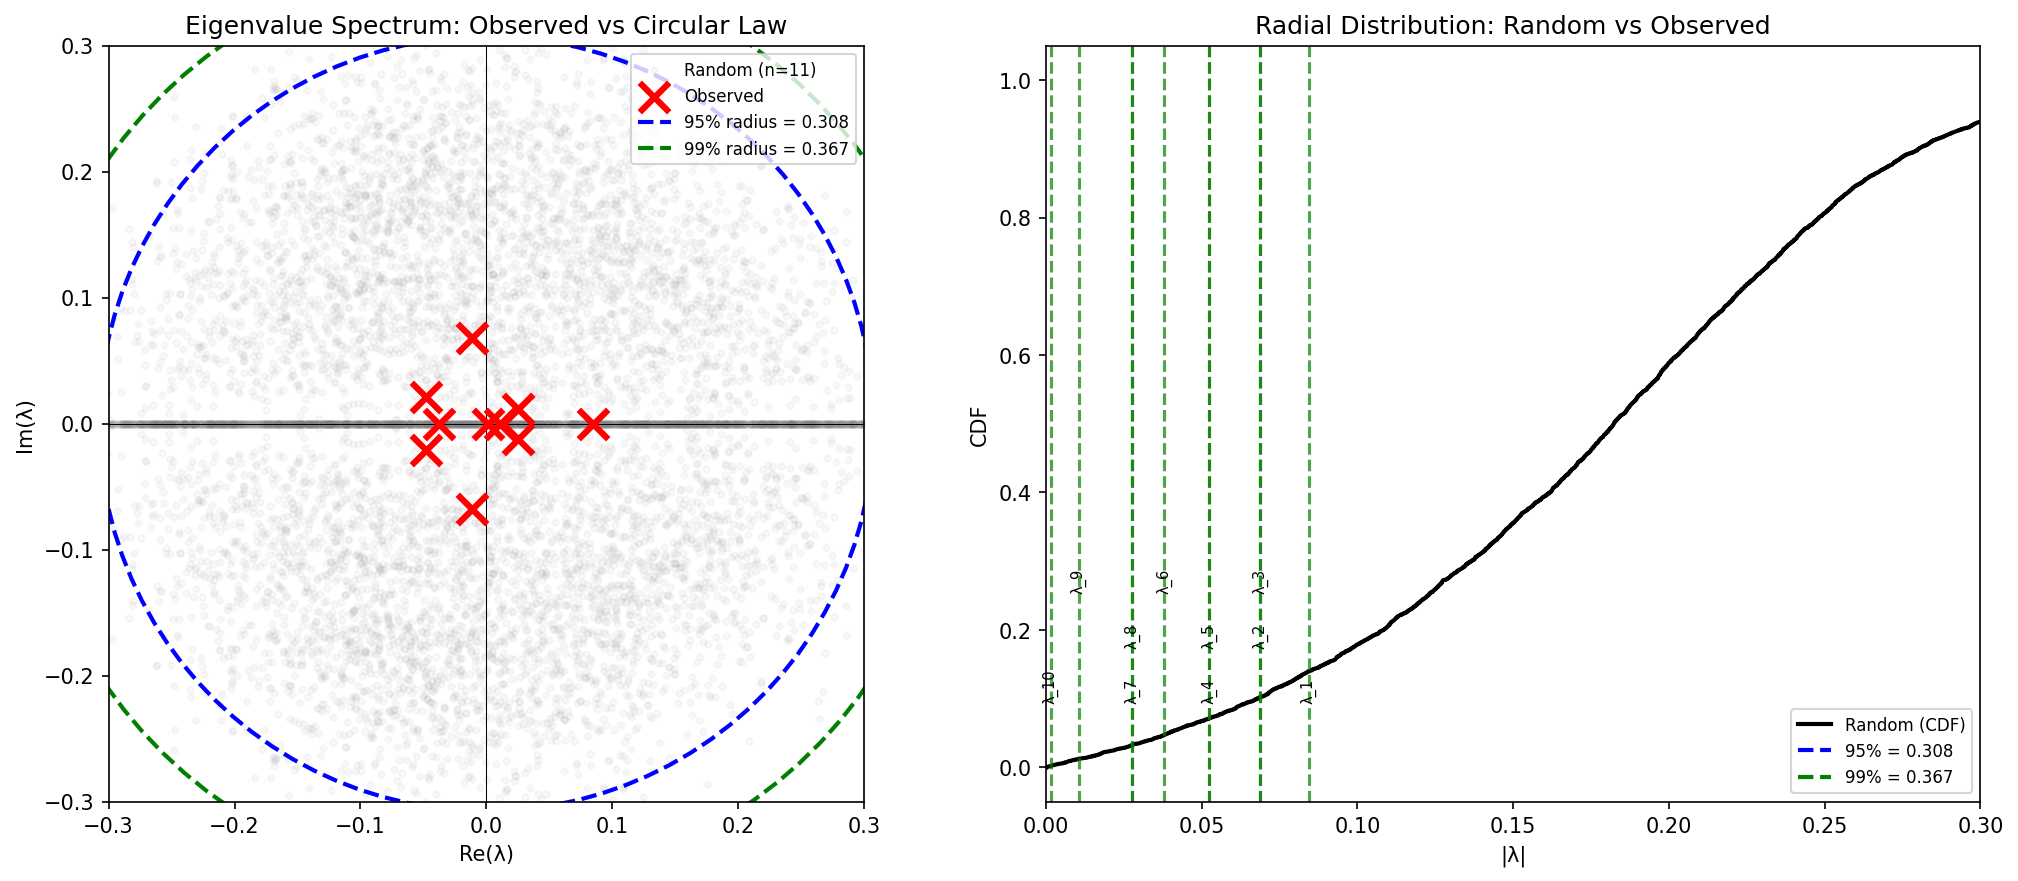
\includegraphics[width=0.95\textwidth]{figures/circular_law_benchmark.png}
\caption{Observed eigenvalues of the daily $\tilde P$ (red crosses) against the circular-law null generated from 1{,}000 Dirichlet-row random stochastic matrices (gray cloud), with 95\% and 99\% radii marked.}
\label{fig:circular}
\end{figure}

\subsection{Permutation bootstrap}

The asymptotic disk radius is an $n\to\infty$ approximation and does not reflect our unequal row sample sizes $n_{i\cdot}$; at $n=11$, edge effects and the specific finite-sample count structure both matter. We therefore also run a permutation bootstrap: shuffle the observed 1{,}644-day laggard sequence (preserving its marginal state frequencies exactly), re-estimate $\tilde P$ with the same $\alpha=1$ smoothing, and recompute its spectrum. Repeating 5{,}000 times yields an exact finite-sample null distribution tailored to our data and estimator, instead of relying on the idealized Dirichlet-row generative assumption.

Table~\ref{tab:bootstrap} reports, for each eigenvalue rank, the empirical p-value $p_k = \Pr(|\lambda_k^{\text{boot}}| \ge |\lambda_k^{\text{obs}}|)$. None reach conventional significance. We do not correct these ten individual $p_k$ for multiple comparisons; since the smallest of them is $p=0.191$, far above any conventional threshold, a correction would only push the values higher and cannot change the conclusion. Three joint tests corroborate: the maximum non-Perron modulus test ($p=0.212$), a trace test on $\sum_k|\lambda_k|^2$ ($p=0.590$), and a complex-eigenvalue-count test ($p=0.952$, observed 3 pairs vs.\ bootstrap mean 3.6 pairs). Figure~\ref{fig:bootstrap} shows the bootstrap null densities for the six largest-modulus eigenvalues against the observed values.

\begin{table}[htbp]\centering
\caption{Permutation bootstrap (5{,}000 reps): observed vs.\ null eigenvalue moduli.}
\label{tab:bootstrap}
\begin{tabular}{lccccc}
\toprule
Rank & $|\lambda|_{\text{obs}}$ & Mean$_{\text{boot}}$ & SD$_{\text{boot}}$ & $p$-value & Signal? \\
\midrule
$\lambda_1$ & 0.0844 & 0.0759 & 0.0118 & 0.212 & no \\
$\lambda_2$ & 0.0688 & 0.0686 & 0.0095 & 0.462 & no \\
$\lambda_3$ & 0.0688 & 0.0618 & 0.0083 & 0.191 & no \\
$\lambda_4$ & 0.0525 & 0.0567 & 0.0079 & 0.692 & no \\
$\lambda_5$ & 0.0525 & 0.0514 & 0.0078 & 0.440 & no \\
$\lambda_6$ & 0.0380 & 0.0459 & 0.0080 & 0.836 & no \\
$\lambda_7$ & 0.0276 & 0.0401 & 0.0083 & 0.933 & no \\
$\lambda_8$ & 0.0276 & 0.0333 & 0.0088 & 0.736 & no \\
$\lambda_9$ & 0.0105 & 0.0251 & 0.0094 & 0.941 & no \\
$\lambda_{10}$ & 0.0015 & 0.0147 & 0.0096 & 0.942 & no \\
\bottomrule
\end{tabular}
\end{table}

\begin{figure}[htbp]\centering
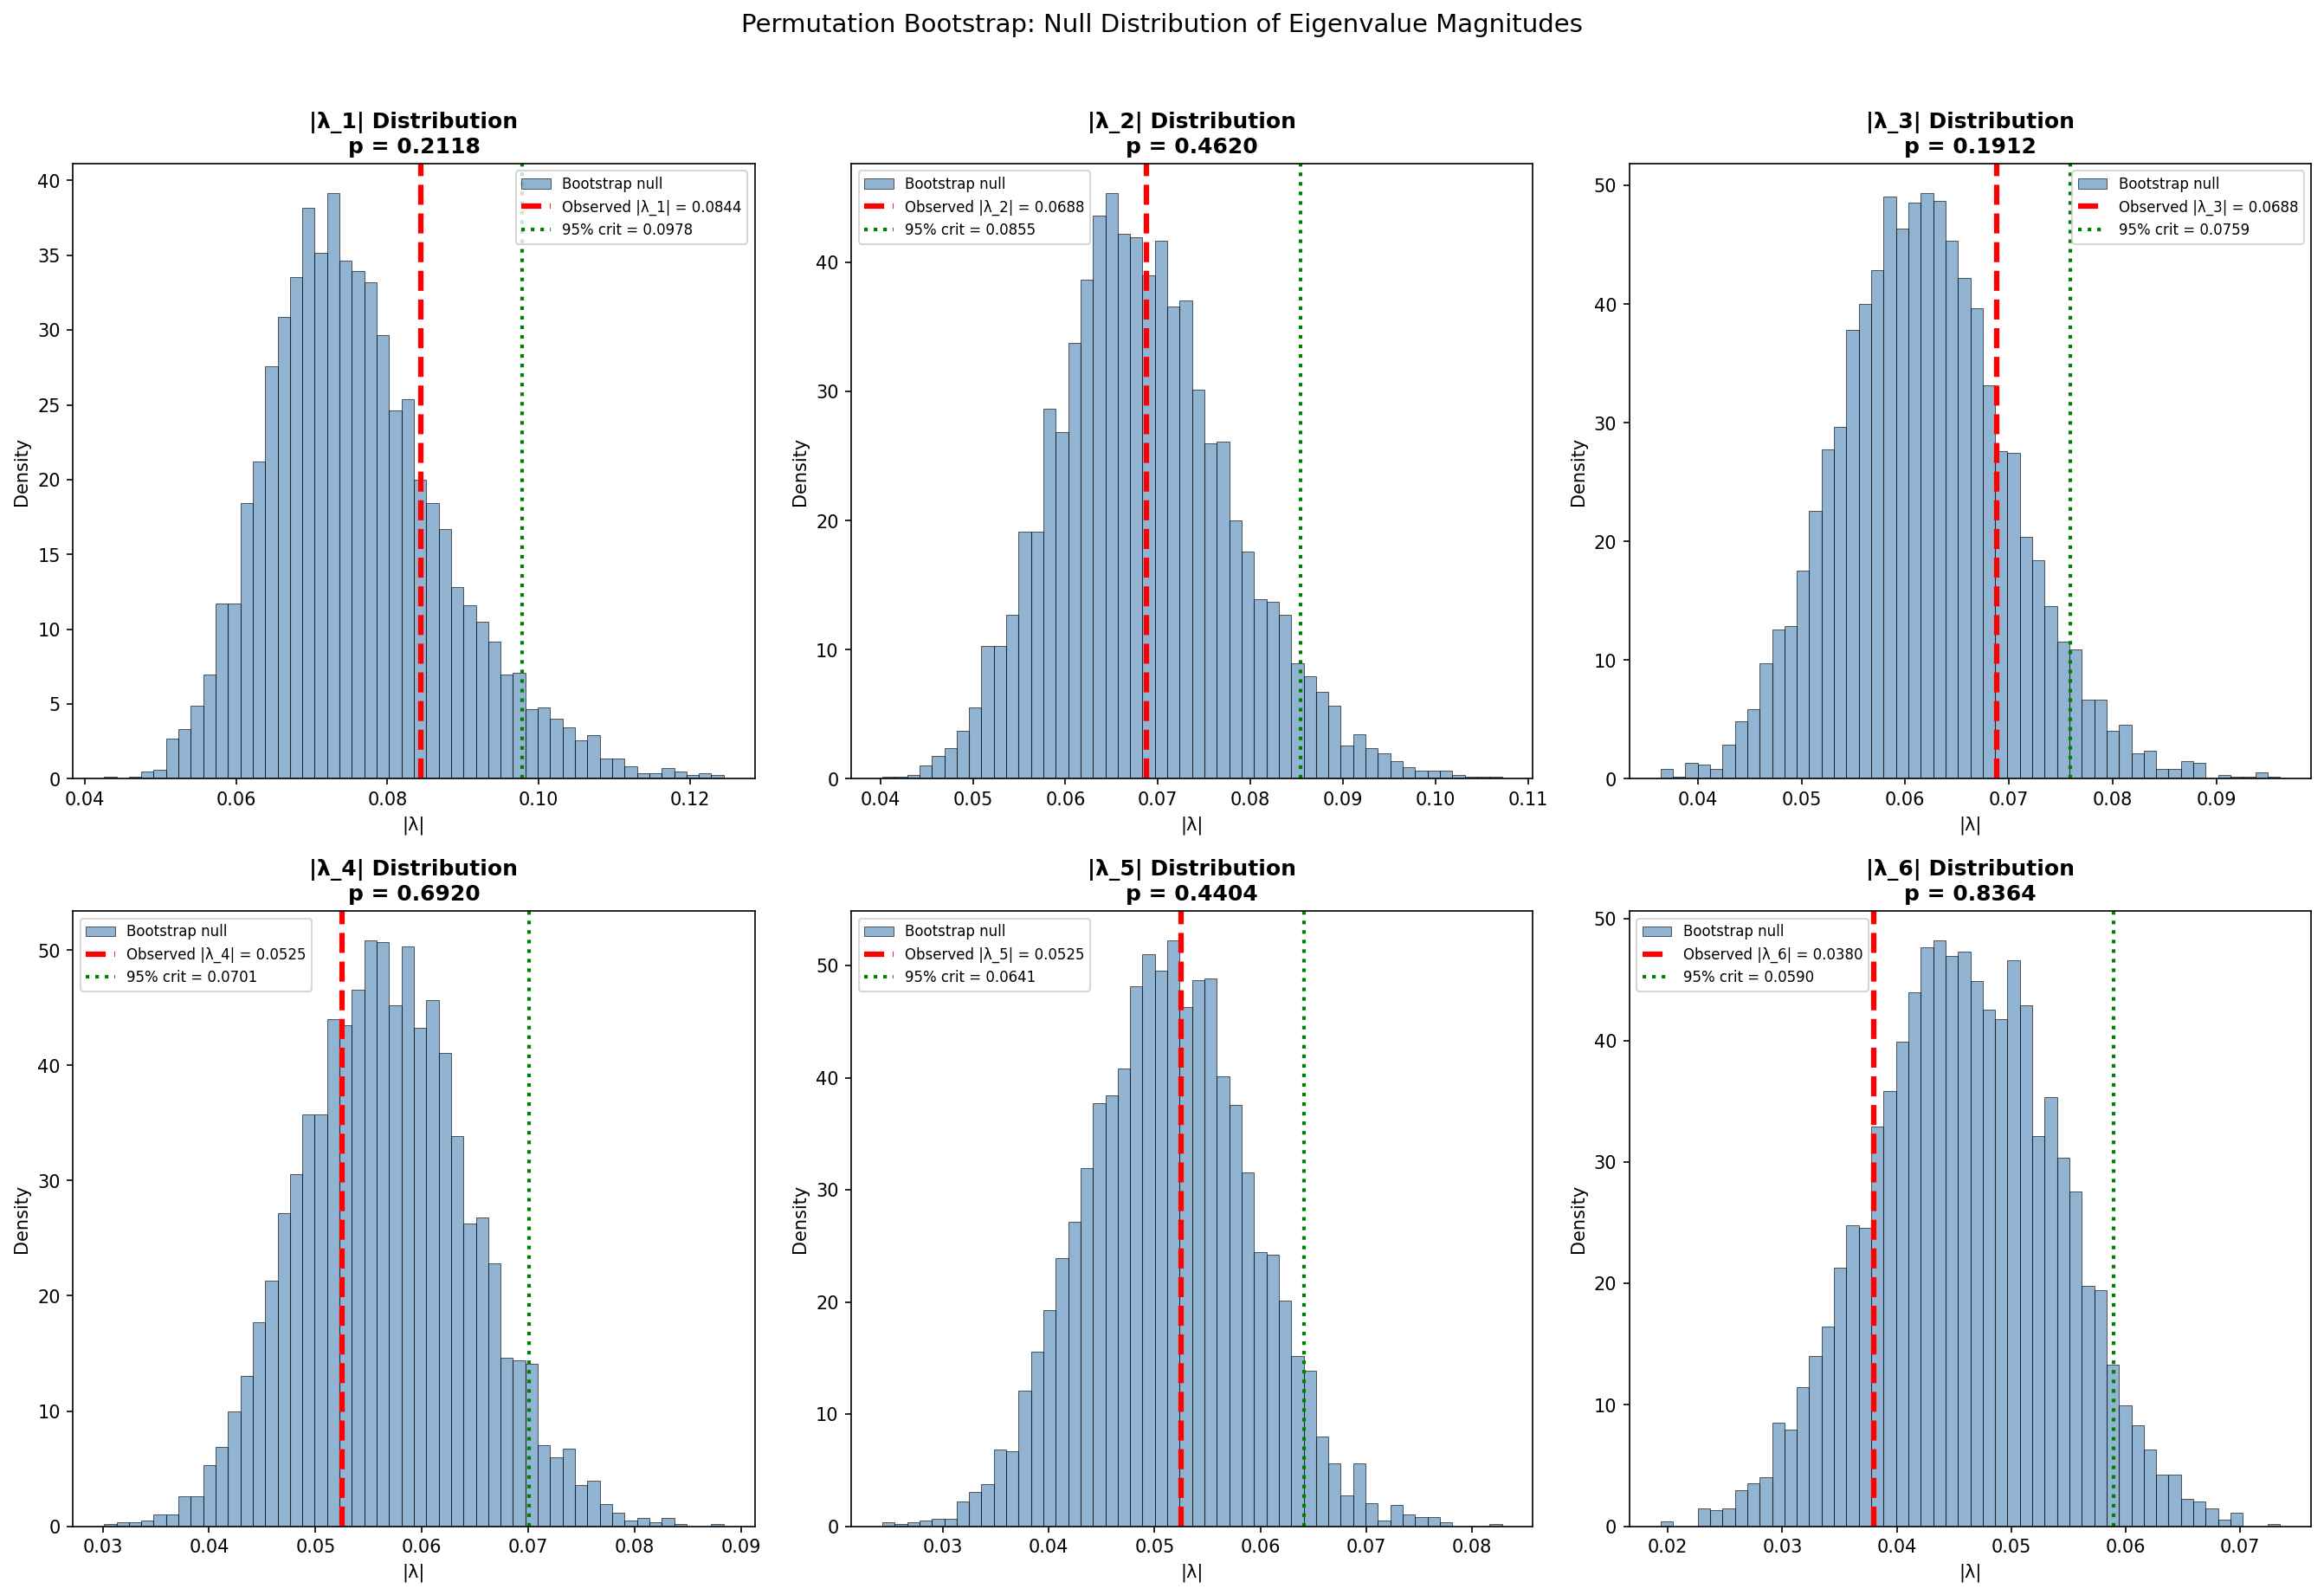
\includegraphics[width=0.95\textwidth]{figures/bootstrap_eigenvalues.png}
\caption{Permutation-bootstrap null distributions (5{,}000 reps) of $|\lambda_1|$ through $|\lambda_6|$, with observed values (dashed red) and 95\% critical values (dotted green).}
\label{fig:bootstrap}
\end{figure}

We conclude that the empirical spectral gap, though real in-sample, is statistically indistinguishable from what an $11\times11$ random stochastic matrix would generate by construction alone. The daily laggard sequence contains no detectable persistence or cyclicality beyond what the row-stochasticity constraint itself induces.

\clearpage
\section{Robustness}
\label{sec:robust}

\subsection{Markov order}

We test order-1 against order-2 dependence via a likelihood-ratio test, comparing $\log \hat L$ under $\hat P_{ij}$ against a second-order model $\hat P_{ijk}$ estimated on 120 of 121 observed $(i,j)$ state pairs. The LR statistic is $2(\ell_1-\ell_0) = 1584.9$ against $df=1090$ ($\ell_0=-3846.8$, $\ell_1=-3054.4$), rejecting order-1 at $p\approx0$. However, AIC and BIC both favor the parsimonious order-1 model (order-1: 110 parameters, AIC $=7913.6$, BIC $=8508.1$; order-2: 1{,}200 parameters, AIC $=8508.7$, BIC $=14{,}993.1$). These results are reconcilable: the LR test is anti-conservative here, because the order-2 alternative has roughly 11$\times$ as many free parameters as observations warrant (Section~\ref{sec:sparsity}), so it will nearly always show a nominal likelihood improvement even under the true order-1 null. The penalized criteria are the appropriate adjudicator, and we retain the order-1 specification used throughout the paper.

\subsection{Time-homogeneity}

We split the sample into crisis sub-periods (COVID-19, February--April 2020; the 2022 rate-hike/Ukraine period, January--June 2022; the March 2023 regional-banking stress episode; 209 of 1{,}644 days, 12.7\%) and the remaining calm days, estimate separate smoothed chains $P_{\text{calm}}, P_{\text{crisis}}$, and compare their joint log-likelihood against a single pooled chain via a likelihood-ratio test. The statistic is $2(\ell_{\text{calm}}+\ell_{\text{crisis}} - \ell_{\text{pooled}}) = 68.1$ against $df=110$, giving $p=0.999$: we fail to reject time-homogeneity. The largest calm-vs-crisis differences (e.g.\ Real Estate$\to$Consumer Discretionary, $+0.110$; Communication$\to$Real Estate, $-0.108$) are individually notable but do not survive as a joint departure from homogeneity. Had homogeneity been rejected, the natural extension would be a regime-switching (hidden Markov) model with a latent volatility state modulating $P$; our result does not require it.

\subsection{Leader-chain robustness check}
\label{sec:leader}

The results above are specific to the \emph{laggard} state definition, $S_t=\arg\min_i r_{i,t}$ (Section~\ref{sec:state}). As a further robustness check, we repeat the full pipeline, transition-matrix estimation, Laplace smoothing, spectral decomposition, circular-law benchmark, and permutation bootstrap, on the complementary \emph{leader} chain, $S_t=\arg\max_i r_{i,t}$, over the same common period (2018-06-20 to 2024-12-31, 1{,}643 transitions).

The leader chain's stationary distribution mirrors the laggard chain's in an interesting way: Energy is again the most frequent state ($\pi^{\text{leader}}_{\text{Energy}}=0.209$, recurring every 4.8 days), and Industrials again the rarest ($\pi^{\text{leader}}_{\text{Industrials}}=0.034$, recurring every 29.9 days). Energy is evidently the most cross-sectionally volatile sector in both directions, not directionally biased, and Industrials the most consistently mid-pack.

Spectrally, the leader chain's second-largest eigenvalue modulus is $|\lambda_1^{\text{leader}}|=0.0772$, giving spectral gap $\gamma^{\text{leader}}=0.9228$, close to the laggard chain's $\gamma=0.9156$, and well inside the $n=11$ circular-law disk of radius $1/\sqrt{11}\approx0.3015$. Table~\ref{tab:leader_bootstrap} reports the 5{,}000-replication permutation bootstrap on the leader-chain spectrum: no individual eigenvalue reaches conventional significance (the smallest is $p=0.098$, for $\lambda_{10}^{\text{leader}}$), and the three joint tests agree (max-modulus $p=0.416$; trace $p=0.243$; complex-eigenvalue-count $p=0.531$, observed 4 pairs against a bootstrap mean of 3.5).

\begin{table}[htbp]\centering
\caption{Leader-chain permutation bootstrap (5{,}000 reps): observed vs.\ null eigenvalue moduli.}
\label{tab:leader_bootstrap}
\begin{tabular}{lccccc}
\toprule
Rank & $|\lambda|_{\text{obs}}$ & Mean$_{\text{boot}}$ & SD$_{\text{boot}}$ & $p$-value & Signal? \\
\midrule
$\lambda_1$ & 0.0772 & 0.0763 & 0.0120 & 0.416 & no \\
$\lambda_2$ & 0.0772 & 0.0691 & 0.0097 & 0.190 & no \\
$\lambda_3$ & 0.0722 & 0.0622 & 0.0084 & 0.120 & no \\
$\lambda_4$ & 0.0547 & 0.0569 & 0.0081 & 0.602 & no \\
$\lambda_5$ & 0.0547 & 0.0514 & 0.0080 & 0.347 & no \\
$\lambda_6$ & 0.0489 & 0.0461 & 0.0081 & 0.353 & no \\
$\lambda_7$ & 0.0489 & 0.0400 & 0.0085 & 0.149 & no \\
$\lambda_8$ & 0.0296 & 0.0333 & 0.0088 & 0.660 & no \\
$\lambda_9$ & 0.0296 & 0.0250 & 0.0095 & 0.317 & no \\
$\lambda_{10}$ & 0.0281 & 0.0146 & 0.0095 & 0.098 & no \\
\bottomrule
\end{tabular}
\end{table}

The leader chain, like the laggard chain, has no eigenvalue surviving either the circular-law or the permutation-bootstrap test. The absence of detectable spectral signal reported in Section~\ref{sec:rmt} is therefore not an artifact of conditioning on the worst performer specifically: it holds symmetrically for the best performer, consistent with the mechanism argument of Section~\ref{sec:mechanism}, which predicts no serial structure regardless of which tail of the daily cross-section is tracked.

\clearpage
\section{Mechanism: Why No Signal?}
\label{sec:mechanism}

The mechanical construction of the underlying products offers a ready explanation for the absence of detectable spectral structure, instead of leaving it as an unexplained null result.

A cap-weighted index tracker requires \emph{no trading} in response to a pure price move: because each constituent's index weight is its market capitalization divided by total index capitalization, a 15\% price decline in one name mechanically reduces its own weight without requiring any rebalancing transaction by the fund. An \emph{equal-weight} fund, by contrast, must periodically buy back down to equal dollar weights: after a 15\% decline, the faller's weight sits below $1/N$, forcing the fund to \emph{buy the faller} --- a mechanical, calendar-driven mean-reversion flow imposed on prices independent of any economic view. Daily-rebalanced \emph{leveraged} products impose the opposite force: to hold constant leverage, a rise in the underlying requires the fund to \emph{increase} dollar exposure, i.e.\ buy the riser, a forced momentum flow.

These two mechanisms have distinct, testable spectral signatures. Equal-weight-style forced mean reversion should manifest as strong \emph{alternation} in the laggard sequence --- a large real, \emph{negative} sub-dominant eigenvalue (the discrete signature of period-2 oscillation: today's laggard tends not to be tomorrow's). Leveraged-style forced momentum should manifest as elevated diagonal (self-transition) mass in $\hat P$ --- a large real, \emph{positive} sub-dominant eigenvalue close to $\lambda_0=1$ (today's laggard tends to remain tomorrow's). A chain with neither mechanical force acting on it has no structural reason to deviate from the row-stochastic random-matrix baseline of Section~\ref{sec:rmt}.

The SPDR Select Sector ETFs used in this paper are cap-weighted, not equal-weight or leveraged. There is accordingly no mechanical rebalancing flow embedded in the product structure that would push the laggard-transition spectrum away from its random-matrix null. The finding of Section~\ref{sec:rmt} --- a real but statistically insignificant spectral gap, with no complex-eigenvalue signal surviving the bootstrap --- is exactly the outcome this mechanism predicts, not a surprising negative result.

\clearpage
\section{Discussion and Limitations}

Reducing an 11-dimensional daily return vector to a single ``worst performer'' label is a coarse summary, and real information is discarded in the collapse; a richer state (e.g.\ joint quintile ranks, or continuous factor loadings) could in principle carry more structure, at the cost of the free-parameter blowup discussed in Section~\ref{sec:sparsity}. The unbalanced panel (Communication Services and Real Estate ETFs launched after 2010) forces a shorter common estimation window (6.5 years) than the full available history; results for those two sectors specifically rest on less data than the rest of the matrix. Finally, the mechanism argument in Section~\ref{sec:mechanism} is specific to the laggard definition and to cap-weighted, non-leveraged products --- it should not be extrapolated to an equal-weight universe, an intraday state definition, or single-stock instead of sector-level aggregation without re-deriving the corresponding spectral prediction.

A further limitation concerns sector definitions themselves: both the GICS sector taxonomy and the constituent holdings of each SPDR Select Sector ETF have changed over 2010--2024 (the 2018 creation of the Communication Services sector, which reclassified several large media and internet names out of Technology and Consumer Discretionary, is the most consequential example). Because we treat each ETF ticker as a fixed proxy for its sector throughout, any such reclassification is implicitly absorbed into that sector's return series, not modeled explicitly. We do not address this here, though it could in principle contribute to the apparent regime stability documented in Section~\ref{sec:robust}, since a sector's underlying composition, not just its relative performance, shifts over the sample.

\clearpage
\section{Conclusion}

Sector rotation is a Markov chain once the state is defined as a single categorical label (here, the daily laggard sector), not as a pairwise conditional-probability table. Doing so on eleven S\&P 500 sector ETFs over 2010--2024 produces an ergodic chain with a real, computable spectral gap ($\gamma=0.916$) and several complex eigenvalue pairs suggestive of short cyclical rotation. Testing that structure against the null model actually appropriate for a row-stochastic matrix --- the circular law for random Markov matrices, not Marchenko--Pastur --- shows none of it survives: every eigenvalue is statistically consistent with a random $11\times11$ stochastic matrix, under both an asymptotic disk-radius approximation and a 5{,}000-replication permutation bootstrap. The same procedure, applied to a hypothetical chain with a genuinely large complex eigenvalue pair, correctly identifies it as signal, confirming the test has power instead of being too weak to detect real structure. The absence of signal in the real data is instead well explained by mechanism: cap-weighted sector ETFs embed no forced rebalancing flow, mean-reverting or momentum-driven, that would imprint serial structure onto which sector leads or lags from one day to the next.

\appendix
\clearpage
\section{Full Transition and Hitting-Time Matrices}
\label{app:matrices}

Sector abbreviations: COMM = Communication, CDIS = Consumer Discretionary, CSTA = Consumer Staples, ENGY = Energy, FINA = Financials, HLTH = Health Care, INDU = Industrials, MATL = Materials, REAL = Real Estate, TECH = Technology, UTIL = Utilities.

\begin{table}[htbp]\centering\scriptsize
\caption{Daily transition counts $n_{ij}$, common period (2018-06-20 to 2024-12-31, 1643 transitions).}
\label{tab:daily_counts}
\resizebox{\textwidth}{!}{
\begin{tabular}{lccccccccccc}
\toprule
From $\backslash$ To & COMM & CDIS & CSTA & ENGY & FINA & HLTH & INDU & MATL & REAL & TECH & UTIL \\
\midrule
COMM & 16 & 14 & 2 & 33 & 4 & 8 & 2 & 9 & 18 & 10 & 18 \\
CDIS & 14 & 13 & 13 & 28 & 5 & 6 & 2 & 5 & 10 & 14 & 10 \\
CSTA & 9 & 4 & 7 & 22 & 7 & 8 & 2 & 8 & 7 & 7 & 26 \\
ENGY & 37 & 20 & 32 & 97 & 20 & 21 & 17 & 18 & 42 & 34 & 49 \\
FINA & 5 & 5 & 8 & 22 & 3 & 5 & 1 & 6 & 10 & 8 & 13 \\
HLTH & 4 & 9 & 7 & 21 & 7 & 7 & 3 & 5 & 13 & 13 & 20 \\
INDU & 3 & 3 & 2 & 11 & 4 & 6 & 0 & 2 & 1 & 4 & 9 \\
MATL & 7 & 7 & 8 & 28 & 7 & 6 & 3 & 3 & 8 & 14 & 7 \\
REAL & 12 & 12 & 8 & 34 & 11 & 14 & 4 & 15 & 11 & 21 & 25 \\
TECH & 13 & 16 & 8 & 42 & 5 & 12 & 4 & 8 & 23 & 17 & 19 \\
UTIL & 14 & 17 & 12 & 49 & 13 & 16 & 7 & 18 & 24 & 26 & 27 \\
\bottomrule
\end{tabular}}
\end{table}

\begin{table}[htbp]\centering\scriptsize
\caption{Daily Laplace-smoothed transition matrix $\tilde P$ ($\alpha=1$), common period.}
\label{tab:daily_ptilde}
\resizebox{\textwidth}{!}{
\begin{tabular}{lccccccccccc}
\toprule
From $\backslash$ To & COMM & CDIS & CSTA & ENGY & FINA & HLTH & INDU & MATL & REAL & TECH & UTIL \\
\midrule
COMM & 0.1172 & 0.1034 & 0.0207 & 0.2345 & 0.0345 & 0.0621 & 0.0207 & 0.0690 & 0.1310 & 0.0759 & 0.1310 \\
CDIS & 0.1145 & 0.1069 & 0.1069 & 0.2214 & 0.0458 & 0.0534 & 0.0229 & 0.0458 & 0.0840 & 0.1145 & 0.0840 \\
CSTA & 0.0847 & 0.0424 & 0.0678 & 0.1949 & 0.0678 & 0.0763 & 0.0254 & 0.0763 & 0.0678 & 0.0678 & 0.2288 \\
ENGY & 0.0955 & 0.0528 & 0.0829 & 0.2462 & 0.0528 & 0.0553 & 0.0452 & 0.0477 & 0.1080 & 0.0879 & 0.1256 \\
FINA & 0.0619 & 0.0619 & 0.0928 & 0.2371 & 0.0412 & 0.0619 & 0.0206 & 0.0722 & 0.1134 & 0.0928 & 0.1443 \\
HLTH & 0.0417 & 0.0833 & 0.0667 & 0.1833 & 0.0667 & 0.0667 & 0.0333 & 0.0500 & 0.1167 & 0.1167 & 0.1750 \\
INDU & 0.0714 & 0.0714 & 0.0536 & 0.2143 & 0.0893 & 0.1250 & 0.0179 & 0.0536 & 0.0357 & 0.0893 & 0.1786 \\
MATL & 0.0734 & 0.0734 & 0.0826 & 0.2661 & 0.0734 & 0.0642 & 0.0367 & 0.0367 & 0.0826 & 0.1376 & 0.0734 \\
REAL & 0.0730 & 0.0730 & 0.0506 & 0.1966 & 0.0674 & 0.0843 & 0.0281 & 0.0899 & 0.0674 & 0.1236 & 0.1461 \\
TECH & 0.0787 & 0.0955 & 0.0506 & 0.2416 & 0.0337 & 0.0730 & 0.0281 & 0.0506 & 0.1348 & 0.1011 & 0.1124 \\
UTIL & 0.0641 & 0.0769 & 0.0556 & 0.2137 & 0.0598 & 0.0727 & 0.0342 & 0.0812 & 0.1068 & 0.1154 & 0.1197 \\
\bottomrule
\end{tabular}}
\end{table}

\begin{table}[htbp]\centering\scriptsize
\caption{Expected hitting times $H_{ij}$ (trading days), daily smoothed chain.}
\label{tab:hitting}
\resizebox{\textwidth}{!}{
\begin{tabular}{lccccccccccc}
\toprule
From $\backslash$ To & COMM & CDIS & CSTA & ENGY & FINA & HLTH & INDU & MATL & REAL & TECH & UTIL \\
\midrule
COMM & 0.0 & 13.5 & 15.7 & 4.5 & 18.4 & 14.8 & 31.4 & 15.8 & 9.3 & 10.1 & 7.5 \\
CDIS & 12.2 & 0.0 & 14.3 & 4.5 & 18.2 & 14.9 & 31.4 & 16.2 & 9.8 & 9.8 & 7.8 \\
CSTA & 12.6 & 14.4 & 0.0 & 4.7 & 17.7 & 14.6 & 31.3 & 15.6 & 9.9 & 10.2 & 6.7 \\
ENGY & 12.5 & 14.2 & 14.7 & 0.0 & 18.0 & 14.9 & 30.6 & 16.1 & 9.5 & 10.0 & 7.5 \\
FINA & 12.9 & 14.1 & 14.6 & 4.5 & 0.0 & 14.8 & 31.4 & 15.7 & 9.5 & 9.9 & 7.3 \\
HLTH & 13.2 & 13.8 & 14.9 & 4.7 & 17.7 & 0.0 & 31.0 & 16.1 & 9.4 & 9.7 & 7.1 \\
INDU & 12.8 & 13.9 & 15.1 & 4.6 & 17.4 & 13.9 & 0.0 & 16.0 & 10.2 & 10.0 & 7.1 \\
MATL & 12.7 & 13.9 & 14.7 & 4.3 & 17.7 & 14.8 & 30.9 & 0.0 & 9.8 & 9.5 & 7.8 \\
REAL & 12.8 & 13.9 & 15.2 & 4.6 & 17.8 & 14.5 & 31.2 & 15.5 & 0.0 & 9.6 & 7.3 \\
TECH & 12.7 & 13.6 & 15.2 & 4.5 & 18.4 & 14.6 & 31.2 & 16.1 & 9.3 & 0.0 & 7.6 \\
UTIL & 12.9 & 13.9 & 15.1 & 4.6 & 17.9 & 14.6 & 31.0 & 15.6 & 9.5 & 9.7 & 0.0 \\
\bottomrule
\end{tabular}}
\end{table}

\clearpage
\section{Worked Toy Example}
\label{app:toy}

This appendix works a small, hand-checkable three-state universe, Technology (T), Financials (F), Energy (E), through the estimation, stationarity, and spectral machinery used in the main text. The source problem set this paper extends posed each concept with its own convenient illustrative matrix, so the three parts below use three different (though comparably sized) transition matrices over the same three states rather than a single matrix carried through all three steps; each part is otherwise self-contained and mirrors the corresponding empirical calculation in the main text.

\subsection{Transition matrix estimation}

Using the 13-period laggard sequence
\begin{equation}
T,\,T,\,T,\,E,\,T,\,F,\,T,\,F,\,E,\,F,\,F,\,T,\,F,
\end{equation}
we tabulate the 12 observed transitions into the count matrix $n_{ij}$ (rows = from, columns = to, order T, F, E):
\begin{equation}
n = \begin{pmatrix} 2 & 3 & 1 \\ 2 & 1 & 1 \\ 1 & 1 & 0 \end{pmatrix}, \qquad n_{T\cdot}=6,\ \ n_{F\cdot}=4,\ \ n_{E\cdot}=2.
\end{equation}
The maximum-likelihood transition matrix $\hat P_{ij} = n_{ij}/n_{i\cdot}$ is
\begin{equation}
\hat P = \begin{pmatrix} 0.333 & 0.500 & 0.167 \\ 0.500 & 0.250 & 0.250 \\ 0.500 & 0.500 & 0.000 \end{pmatrix},
\end{equation}
with each row summing to 1 by construction. The entry $\hat P_{EE}=0$ (Energy never remained the laggard two weeks running) is a sampling artifact of a 13-observation sample, not evidence that the transition is structurally impossible: with only 2 departures from state $E$, a single additional week of data could easily produce $E\to E$.

Applying Laplace smoothing ($\alpha=1$) to the Energy row ($n_{E\cdot}=2$, $n=3$ states) gives
\begin{equation}
\tilde P_{E,\cdot} = \left(\frac{1+1}{2+3},\ \frac{1+1}{2+3},\ \frac{0+1}{2+3}\right) = (0.400,\ 0.400,\ 0.200)
\end{equation}
in $(T,F,E)$ order, replacing the zero with a small positive probability so that the resulting chain can be irreducible (Section~\ref{sec:sparsity}).

\subsection{Stationary distribution and recurrence}

For the $3\times3$ matrix over $(T,F,E)$
\begin{equation}
P = \begin{pmatrix} 0.50 & 0.50 & 0.00 \\ 0.25 & 0.50 & 0.25 \\ 0.00 & 0.50 & 0.50 \end{pmatrix},
\end{equation}
solving $\pi P = \pi$ with $\sum_i \pi_i=1$ gives $\pi_T = \pi_E = \tfrac12 \pi_F$ and hence
\begin{equation}
\pi = (\pi_T,\pi_F,\pi_E) = (0.25,\ 0.50,\ 0.25).
\end{equation}
By Kac's lemma, $\mathbb E[T_{ii}]=1/\pi_i$ \cite{kemenysnell1976}, so the mean recurrence times are $(1/\pi_T, 1/\pi_F, 1/\pi_E) = (4,\ 2,\ 4)$ periods: Financials is the laggard most often in steady state and recurs to that role fastest, every 2 periods on average.

\subsection{Spectral gap and cyclical structure}

Consider a different, approximately cyclic estimated $3\times3$ chain with eigenvalues $\lambda_1=1$, $\lambda_{2,3} = -0.35 \pm 0.606i$. The modulus is
\begin{equation}
|\lambda_2| = \sqrt{0.35^2 + 0.606^2} = \sqrt{0.4897} \approx 0.700,
\end{equation}
giving spectral gap $g = 1-|\lambda_2| \approx 0.300$ and relaxation time $\approx 1/g \approx 3.3$ periods --- a slowly-decaying, persistent pattern. The eigenvalue's argument is
\begin{equation}
\theta = \arg(\lambda_2) = \pi - \arctan\!\left(\frac{0.606}{0.35}\right) \approx \frac{2\pi}{3} \ \text{rad} = 120^\circ,
\end{equation}
which is exact to four significant figures: $0.6998\cdot(\cos 120^\circ, \sin 120^\circ) = (-0.350, 0.606)$. The implied rotation period is
\begin{equation}
\frac{2\pi}{\theta} = 3.00 \ \text{periods},
\end{equation}
an exact 3-cycle (e.g.\ $T\to F\to E\to T$). A complex eigenvalue pair is the signature of a \emph{directional}, multi-state cycle; it is structurally invisible to a symmetric object like a correlation matrix, because a symmetric matrix's eigenvalues are always real --- correlation captures co-movement magnitude but cannot encode that $A$ tends to lead $B$ rather than the reverse. Only an asymmetric, directional transition matrix can carry that information. This example is revisited in Section~\ref{sec:rmt} to confirm the random-matrix test correctly flags it as signal, in contrast with the empirical (no-signal) result on the real 11-sector chain.

\begin{thebibliography}{9}

\bibitem{hamilton1989}
Hamilton, J. D. (1989).
A new approach to the economic analysis of nonstationary time series and the business cycle.
\textit{Econometrica}, 57(2), 357--384.

\bibitem{moskowitzgrinblatt1999}
Moskowitz, T. J., \& Grinblatt, M. (1999).
Do industries explain momentum?
\textit{The Journal of Finance}, 54(4), 1249--1290.

\bibitem{jacobsenetal2009}
Jacobsen, B., Stangl, J. S., \& Visaltanachoti, N. (2009).
Sector rotation across the business cycle.
Working paper, SSRN 1467457.

\bibitem{molchanovstangl2024}
Molchanov, A., \& Stangl, J. (2024).
The myth of business cycle sector rotation.
\textit{International Journal of Finance \& Economics}, 29(4), 4419--4442.

\bibitem{lalouxetal1999}
Laloux, L., Cizeau, P., Bouchaud, J.-P., \& Potters, M. (1999).
Noise dressing of financial correlation matrices.
\textit{Physical Review Letters}, 83(7), 1467--1470.

\bibitem{plerouetal2000}
Plerou, V., Gopikrishnan, P., Rosenow, B., Amaral, L. A. N., \& Stanley, H. E. (2000).
Random matrix theory approach to financial cross-correlations.
\textit{Physica A}, 287(3--4), 374--382.

\bibitem{bouchaudpotters2009}
Bouchaud, J.-P., \& Potters, M. (2009).
Financial applications of random matrix theory: a short review.
arXiv:0910.1205.

\bibitem{bordenave2012}
Bordenave, C., Caputo, P., \& Chafa\"i, D. (2012).
Circular law theorem for random Markov matrices.
\textit{Probability Theory and Related Fields}, 152(3--4), 751--779.

\bibitem{marchenkopastur1967}
Marchenko, V. A., \& Pastur, L. A. (1967).
Distribution of eigenvalues for some sets of random matrices.
\textit{Matematicheskii Sbornik}, 114(4), 507--536.

\bibitem{seneta2006}
Seneta, E. (2006).
\textit{Non-negative Matrices and Markov Chains} (2nd ed.).
Springer.

\bibitem{kemenysnell1976}
Kemeny, J. G., \& Snell, J. L. (1976).
\textit{Finite Markov Chains}.
Springer-Verlag.

\bibitem{levinperes2017}
Levin, D. A., Peres, Y., \& Wilmer, E. L. (2017).
\textit{Markov Chains and Mixing Times} (2nd ed.).
American Mathematical Society.

\bibitem{norris1998}
Norris, J. R. (1998).
\textit{Markov Chains}.
Cambridge University Press.

\bibitem{crsp}
Center for Research in Security Prices (CRSP), University of Chicago Booth School of Business.
Daily Stock File, accessed via Wharton Research Data Services (WRDS), 2025.

\end{thebibliography}

\end{document}
